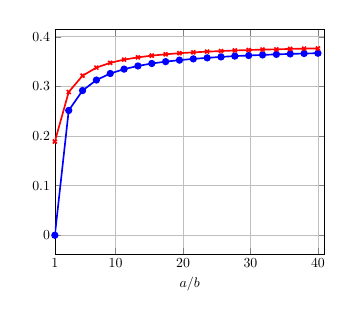
\begin{tikzpicture}[scale=0.5]
\begin{axis}[xlabel=$a/b$,ymajorgrids=true,xmajorgrids=true,xmin=1,xmax=41,xtick={1,10,20,30,40}]
%%%%%%%%%%% NATURAL CONFIGURATION
\addplot[Blue,mark=*,very thick] coordinates {(1.0,1.0000100001e-05) (3.05263157895,0.251417251015) (5.10526315789,0.291564494592) (7.15789473684,0.312731548368) (9.21052631579,0.325871679769) (11.2631578947,0.334744400076) (13.3157894737,0.341153937855) (15.3684210526,0.346100303108) (17.4210526316,0.349818235024) (19.4736842105,0.352866686562) (21.5263157895,0.355403027714) (23.5789473684,0.357460416709) (25.6315789474,0.359358330425) (27.6842105263,0.36100571532) (29.7368421053,0.362198358826) (31.7894736842,0.363357317784) (33.8421052632,0.364483118515) (35.8947368421,0.365412075173) (37.9473684211,0.366195767221) (40.0,0.366803668037) };
%%%%%%%%%%% MODIFIED CONFIGURATION
\addplot[Red,mark=x,very thick] coordinates {(1.0,0.188871888719) (3.05263157895,0.288690255324) (5.10526315789,0.321481635869) (7.15789473684,0.337784430476) (9.21052631579,0.347424526877) (11.2631578947,0.353891959972) (13.3157894737,0.358464637278) (15.3684210526,0.361929935089) (17.4210526316,0.364626277842) (19.4736842105,0.366887879405) (21.5263157895,0.368534211658) (23.5789473684,0.369957383784) (25.6315789474,0.371148974648) (27.6842105263,0.372356355142) (29.7368421053,0.373201100432) (31.7894736842,0.374165846922) (33.8421052632,0.374635851622) (35.8947368421,0.375462701995) (37.9473684211,0.376062181674) (40.0,0.376403764038) };
\end{axis}
\end{tikzpicture}
%%% Local Variables:
%%% mode: latex
%%% TeX-master: "../../mainManuscript"
%%% End:
